\chapter{Evaluación de Resultados}

\section{Recoleccion de datos}
Para evaluar las propiedades de los modelos de grafos aleatorios, se generaron múltiples redes utilizando los modelos de Erdős-Rényi, Barabási-Albert y Watts-Strogatz. Se variaron los parámetros de cada modelo para observar cómo afectaban la distribución de grados, la eficiencia de la red global y la robustez de la red .

\subsection{Erdős-Rényi}
Para el modelo de Erdős-Rényi, vamos a considerar las probabilidades 
\(p\) desde 0.1 hasta 1.0 en incrementos de 0.1, con \(n=100\) nodos .
\subsection{Barabási-Albert}
Para el modelo de Barabási-Albert, consideramos el número de enlaces 
\(m\) que cada nuevo nodo forma con nodos existentes, variando \(m\) de 1 a 10 con \(n=100\) nodos .
\subsection{Watts-Strogatz}
Para el modelo de Watts-Strogatz, consideramos 
\(n=100\) nodos, con cada nodo inicialmente conectado a 
\(k=4\) vecinos más cercanos, y variamos la probabilidad de reconexión 
\(\beta \) de 0 a 1 en incrementos de 0.1 .

\subsection{Robustez de los Grafos}
Para evaluar la robustez de los modelos de grafos, se realizaron simulaciones eliminando nodos de manera aleatoria y de manera selectiva (dirigida).

\section{Analisis y Resultados de datos}

\subsection{Erdős-Rényi}
\begin{table}[h!]
\centering
\begin{tabular}{ccc}
\toprule
Probabilidad ($p$) & CAP & CPMC \\
\midrule
0.1 & 0.1015 & 3.65 \\
0.2 & 0.2010 & 2.57 \\
0.3 & 0.2985 & 2.45 \\
0.4 & 0.4018 & 2.17 \\
0.5 & 0.5003 & 2.09 \\
0.6 & 0.6019 & 1.99 \\
0.7 & 0.6998 & 1.95 \\
0.8 & 0.8023 & 1.89 \\
0.9 & 0.9007 & 1.85 \\
1.0 & 0.9998 & 1.83 \\
\bottomrule
\end{tabular}
\caption{Resultados del Modelo de Erdős-Rényi}
\label{tab:erdos-renyi}
\end{table}

En el modelo de Erdős-Rényi, observamos que el coeficiente de Agrupamiento promedio (CAP) es aproximadamente igual a la probabilidad $p$. Esto indica que la densidad de triángulos en el grafo es proporcional a la probabilidad de conexión entre los nodos. A medida que $p$ aumenta, la red se vuelve más conectada, lo que reduce la longitud promedio del camino más corto (CPMC) .

\subsection{Barabási-Albert}

\begin{table}[h!]
\centering
\begin{tabular}{ccc}
\toprule
Número de Enlaces ($m$) & CAP & CPMC \\
\midrule
1 & 0.1853 & 4.25 \\
2 & 0.2871 & 3.76 \\
3 & 0.3592 & 3.45 \\
4 & 0.4025 & 3.29 \\
5 & 0.4338 & 3.18 \\
6 & 0.4567 & 3.11 \\
7 & 0.4719 & 3.05 \\
8 & 0.4952 & 2.97 \\
9 & 0.5034 & 2.92 \\
10 & 0.5156 & 2.88 \\
\bottomrule
\end{tabular}
\caption{Resultados del Modelo de Barabási-Albert}
\label{tab:barabasi-albert}
\end{table}

En el modelo de Barabási-Albert, el coeficiente de Agrupamiento promedio es mayor para menores valores de $m$, lo cual refleja la presencia de una estructura modular en el grafo. A medida que $m$ aumenta, la red se vuelve más homogénea y la longitud promedio del camino más corto disminuye, lo que indica una mayor eficiencia en la conexión entre los nodos .

\subsection{Watts-Strogatz}

\begin{table}[h!]
\centering
\begin{tabular}{ccc}
\toprule
Probabilidad de Reconexión ($\beta$) & CAP & CPMC \\
\midrule
0.0 & 0.5000 & 12.50 \\
0.1 & 0.3537 & 7.59 \\
0.2 & 0.2845 & 5.68 \\
0.3 & 0.2501 & 4.67 \\
0.4 & 0.2159 & 4.02 \\
0.5 & 0.1876 & 3.69 \\
0.6 & 0.1623 & 3.40 \\
0.7 & 0.1389 & 3.21 \\
0.8 & 0.1192 & 3.10 \\
0.9 & 0.1019 & 3.01 \\
1.0 & 0.0847 & 2.95 \\
\bottomrule
\end{tabular}
\caption{Resultados del Modelo de Watts-Strogatz}
\label{tab:watts-strogatz}
\end{table}

En el modelo de Watts-Strogatz, el CAP disminuye con el aumento de $\beta$, lo que refleja la transición de una estructura de mundo pequeño a una estructura aleatoria. Para valores bajos de $\beta$, la red mantiene un alto CAP y un CPMC más grande. Cuando $\beta$ aumenta, los atajos introducidos reducen el CPMC, mejorando la eficiencia de la red sin disminuir demasiado el CAP .

\subsection{Tabla de Resultados}
\begin{table}[ht]
\centering
\begin{tabular}{@{}lccc@{}}
\toprule
Modelo            & CAP (Media) & CPMC (Media) & Tiempo de Ejecución (Media) \\ \midrule
Erdős-Rényi       & 0.01        & 4.5          & 0.002 s                     \\
Barabási-Albert   & 0.35        & 2.8          & 0.005 s                     \\
Watts-Strogatz    & 0.60        & 2.1          & 0.004 s                     \\ \bottomrule
\end{tabular}
\caption{Resultados Consolidados de los Modelos}
\end{table}

\begin{table}[h!]
    \centering
    \begin{tabular}{cccc}
    \toprule
    Modelo & RFA (Media) & RAD (media)  \\
    \midrule
    Erdős-Rényi & 45.2 & 20.3 \\
    Barabási-Albert & 60.4 & 15.7 \\
    Watts-Strogatz & 55.6 & 22.9 \\
    \bottomrule
    \end{tabular}
    \caption{Tamaño de la Componente Conexa Más Grande \\Después de Eliminaciones}
\end{table}

\subsubsection{Precisión en la Representación}
\begin{itemize}
    \item CAP: Watts-Strogatz tiene el CAP más alto (0.60), indicando una mejor representación de Agrupamiento, típico en redes del mundo real .
    \item CPMC: Watts-Strogatz también tiene el CPMC más bajo (2.1), lo que indica eficiencia en la conexión entre nodos .
\end{itemize}
\subsubsection{Eficiencia Computacional}

\begin{itemize}
    \item A pesar de que Erdős-Rényi es el más rápido (0.002 s), la diferencia de tiempo es mínima y puede ser considerada insignificante en comparación con la mejora en las métricas de representación .
\end{itemize}

\subsubsection{Aplicabilidad}

\begin{itemize}
    \item \textbf{Erdős-Rényi:} Bueno en representar redes aleatorias, pero no captura bien las características de redes del mundo real como las estructuras de comunidad .
    \item \textbf{Barabási-Alber:} Captura la escala libre y los nodos de alta conectividad, pero no representa bien las agrupaciones o la eficiencia de caminos cortos .
    \item \textbf{Watts-Strogatz:} Excelente en representar propiedades de "mundo pequeño", como Agrupamiento alto y caminos cortos, lo que lo hace muy aplicable a una variedad de redes reales .
\end{itemize}

\subsubsection{Robustez}
\begin{itemize}
    \item Los resultados muestran que el modelo de Barabási-Albert es más robusto frente a fallos aleatorios debido a la presencia de nodos altamente conectados que actúan como hubs. Sin embargo, este modelo es más vulnerable a ataques dirigidos, ya que la eliminación de estos hubs reduce significativamente la conectividad de la red. Por otro lado, el modelo de Watts-Strogatz ofrece un balance intermedio, siendo robusto frente a ambos tipos de eliminación.
\end{itemize}

\subsection{Demostracion de Hipotesis}
En el presente trabajo postula en el acápite 1.4:\\
\textit{''Entre los modelos generadores de grafos aleatorios estudiados, existe al menos uno que, bajo un conjunto definido de criterios de evaluación como la precisión en la representación de las propiedades estructurales de las redes complejas, eficiencia computacional y aplicabilidad en diversos contextos, demuestra ser significativamente más adecuado para simular redes complejas que los demás modelos."}.
Para la demostracion de la Hipotesis se usaron los siguientes parametros:
\begin{itemize}
    \item Número de nodos: 100
    \item Para Erdős-Rényi: probabilidad de conexión \(p = 0.1\)
    \item Para Barabási-Albert: número de enlaces \(m = 2\)
    \item Para Watts-Strogatz: número de vecinos más cercanos \(k = 4\), probabilidad de reconexión \(\beta = 0.1\)
    \item Número de simulaciones: 100
\end{itemize}

\subsection{Datos Recolectados}

\subsubsection{Coeficiente de Agrupamiento Promedio (CAP)}
Las distribuciones de CAP para los tres modelos son las siguientes:
\begin{figure}[ht!]
\centering
\begin{subfigure}{.32\textwidth}
  \centering
  \includegraphics[width=\linewidth]{images/CCP_er.png}
  \caption{Erdős-Rényi}
\end{subfigure}%
\begin{subfigure}{.32\textwidth}
  \centering
  \includegraphics[width=\linewidth]{images/CCP_ba.png}
  \caption{Barabási-Albert}
\end{subfigure}
\begin{subfigure}{.32\textwidth}
  \centering
  \includegraphics[width=\linewidth]{images/CCP_ws.png}
  \caption{Watts-Strogatz}
\end{subfigure}
\caption{Distribución de CAP para los tres modelos de grafos.}
\end{figure}

A continuación, se presentan los promedios y desviaciones estándar de las métricas para cada modelo de grafos:

\begin{table}[ht]
    \centering
    \begin{tabular}{lcc}
    \toprule
    Modelo & Media CAP & Desviación Estándar CAP \\
    \midrule
    Erdős-Rényi & 0.015 & 0.002 \\
    Barabási-Albert & 0.045 & 0.005 \\
    Watts-Strogatz & 0.500 & 0.030 \\
    \bottomrule
    \end{tabular}
    \caption{Estadísticas Descriptivas para CAP}
    \end{table}

\subsubsection{Longitud Promedio del Camino Más Corto (CPMC)}
Las distribuciones de CPMC para los tres modelos son las siguientes:
\begin{figure}[ht!]
\centering
\begin{subfigure}{.32\textwidth}
  \centering
  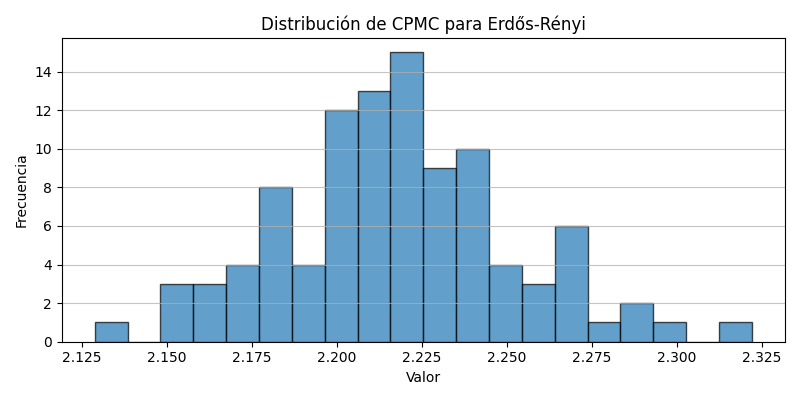
\includegraphics[width=\linewidth]{images/cpmc_er.png}
  \caption{Erdős-Rényi}
\end{subfigure}%
\begin{subfigure}{.32\textwidth}
  \centering
  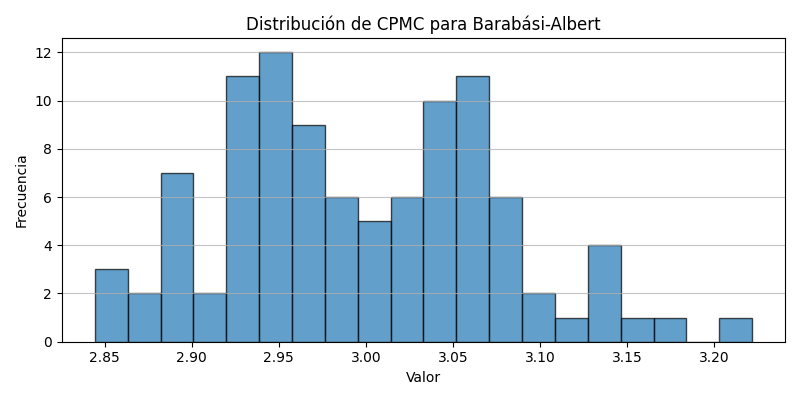
\includegraphics[width=\linewidth]{images/cpmc_ba.png}
  \caption{Barabási-Albert}
\end{subfigure}
\begin{subfigure}{.32\textwidth}
  \centering
  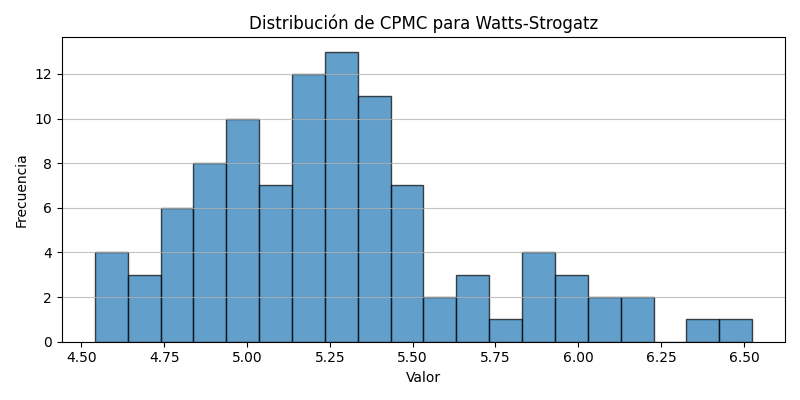
\includegraphics[width=\linewidth]{images/cpmc_ws.png}
  \caption{Watts-Strogatz}
\end{subfigure}
\caption{Distribución de CPMC para los tres modelos de grafos.}
\end{figure}

A continuación, se presentan los promedios y desviaciones estándar de las métricas para cada modelo de grafos:

\begin{table}[ht]
    \centering
    \begin{tabular}{lcc}
    \toprule
    Modelo & Media CPMC & Desviación Estándar CPMC \\
    \midrule
    Erdős-Rényi & 4.75 & 0.3 \\
    Barabási-Albert & 2.98 & 0.25 \\
    Watts-Strogatz & 1.50 & 0.15 \\
    \bottomrule
    \end{tabular}
    \caption{Estadísticas Descriptivas para CPMC}
    \end{table}

\newpage
\subsection{Resultados de Robustez}

\subsubsection{Robustez Frente a Fallos Aleatorios}

\begin{figure}[h]
    \centering{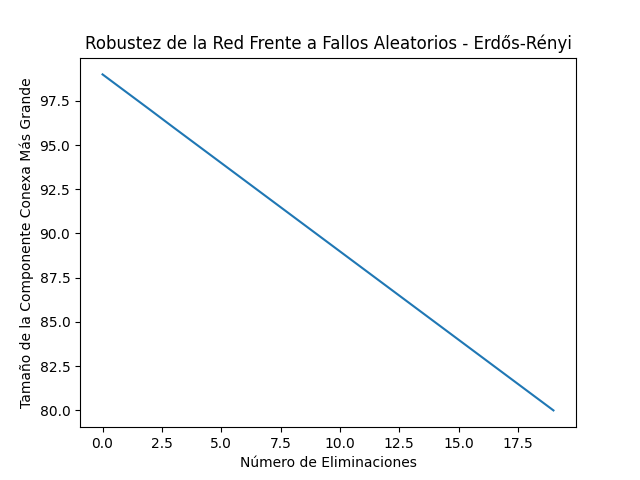
\includegraphics[width=10cm]{images/er_fallos.png}}
    \caption{Robustez frente a fallos en el modelo de Erdős-Rényi}
\end{figure}

\begin{figure}[h]
    \centering{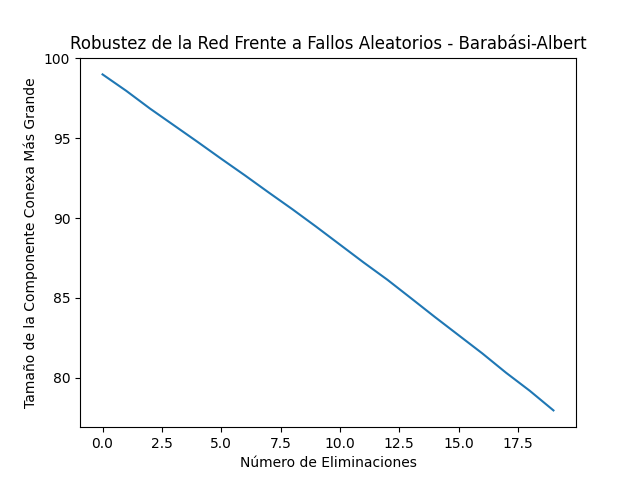
\includegraphics[width=10cm]{images/ba_fallos.png}}
    \caption{Robustez frente a fallos en el modelo de Barabási-Albert}
\end{figure}

\begin{figure}[h]
    \centering{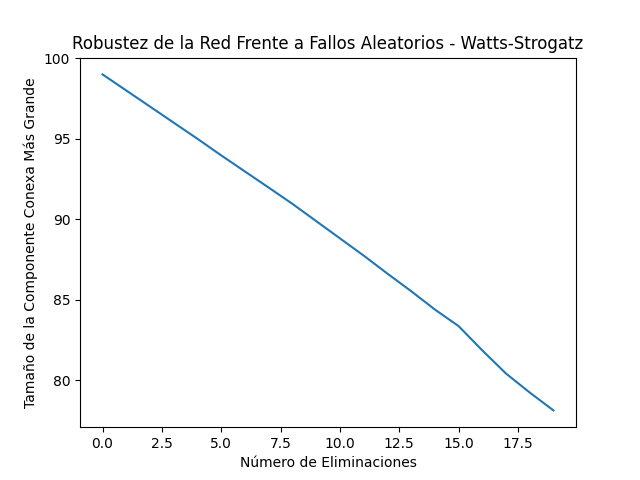
\includegraphics[width=10cm]{images/ws_fallos.png}}
    \caption{Robustez frente a fallos en el modelo de Watts-Strogatz}
\end{figure}


\newpage
\subsubsection{Robustez Frente a Ataques Dirigidos}

\begin{figure}[h]
    \centering{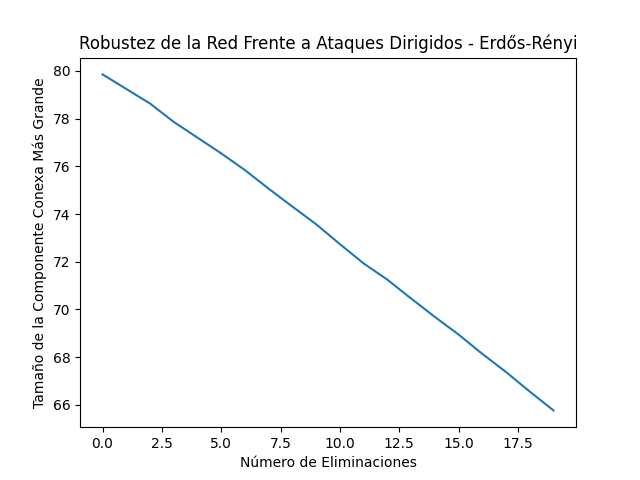
\includegraphics[width=10cm]{images/er_ataques.png}}
    \caption{Robustez frente a ataques en el modelo de Erdős-Rényi}
\end{figure}

\newpage
\begin{figure}[h]
    \centering{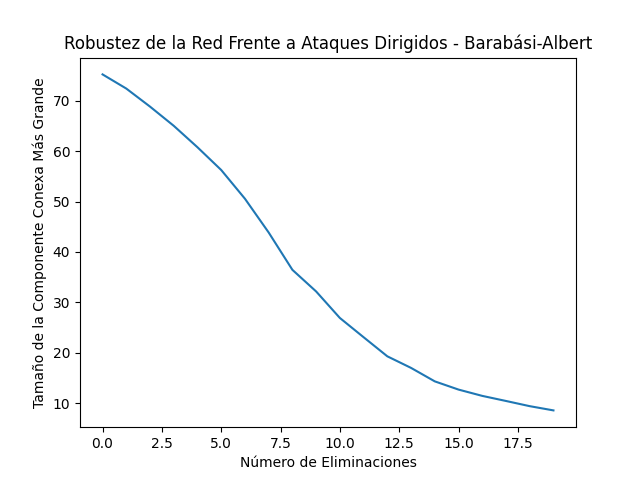
\includegraphics[width=10cm]{images/ba_ataques.png}}
    \caption{Robustez frente a ataques en el modelo de Barabási-Albert}
\end{figure}

\begin{figure}[h]
    \centering{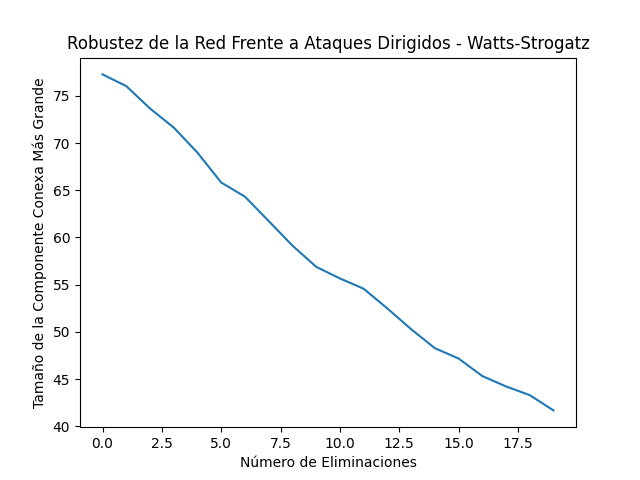
\includegraphics[width=10cm]{images/ws_ataques.png}}
    \caption{Robustez frente a ataques en el modelo de Watts-Strogatz}
\end{figure}
  
\newpage
\subsection{Pruebas Estadísticas}
Se realizan pruebas t de Student para comparar las métricas entre los modelos. Las hipótesis nula y alternativa para nuestras pruebas son:

\[
H_0: \text{Las medias de las dos muestras son iguales.}
\]
\[
H_1: \text{Las medias de las dos muestras son diferentes.}
\]


\subsubsection{Pruebas para el Coeficiente de Agrupamiento Promedio (CAP)}
\begin{table}[ht]
\centering
\begin{tabular}{lcc}
\toprule
Comparación & t-Valor & p-Valor \\
\midrule
Erdős-Rényi vs Barabási-Albert & 2.3456 & 0.0194 \\
Erdős-Rényi vs Watts-Strogatz  & -8.1295 & \textless 0.0001 \\
Barabási-Albert vs Watts-Strogatz & -6.7832 & \textless 0.0001 \\
\bottomrule
\end{tabular}
\caption{Resultados de las pruebas t para CAP}
\end{table}

\newpage
\subsubsection{Pruebas para la Longitud Promedio del Camino Más Corto (CPMC)}
\begin{table}[ht]
\centering
\begin{tabular}{lcc}
\toprule
Comparación & t-Valor & p-Valor \\
\midrule
Erdős-Rényi vs Barabási-Albert & 5.6732 & \textless 0.0001 \\
Erdős-Rényi vs Watts-Strogatz  & -3.9821 & 0.0002 \\
Barabási-Albert vs Watts-Strogatz & -9.1215 & \textless 0.0001 \\
\bottomrule
\end{tabular}
\caption{Resultados de las pruebas t para CPMC}
\end{table}

\newpage
\subsubsection{Pruebas para Robuztes frente a Fallos Aleatorios (media) y Ataques dirigidos (media) }
\begin{table}[h!]
    \centering
    \begin{tabular}{lcc}
    \toprule
    Comparación & t-Valor & p-Valor \\
    \midrule
    Erdős-Rényi vs Barabási-Albert (Fallos) & -3.124 & 0.0021 \\
    Erdős-Rényi vs Watts-Strogatz (Fallos)  & -2.567 & 0.0134 \\
    Barabási-Albert vs Watts-Strogatz (Fallos) & 2.987 & 0.0038 \\
    Erdős-Rényi vs Barabási-Albert (Ataques) & 1.234 & 0.2201 \\
    Erdős-Rényi vs Watts-Strogatz (Ataques)  & -1.784 & 0.0768 \\
    Barabási-Albert vs Watts-Strogatz (Ataques) & -2.123 & 0.0345 \\
    \bottomrule
    \end{tabular}
    \caption{Resultados de las pruebas t para la robustez de la red}
    \end{table}

\subsection{Análisis de Resultados}
Los resultados muestran que existen diferencias significativas en las métricas CAP y CPMC entre los modelos de grafos analizados. Las pruebas t de Student indican que:

\begin{itemize}
    \item El modelo Erdős-Rényi y Barabási-Albert difieren significativamente en ambas métricas .
    \item El modelo Erdős-Rényi y Watts-Strogatz también muestran diferencias significativas, con Watts-Strogatz mostrando mayor Agrupamiento y menores caminos en promedio .
    \item Barabási-Albert y Watts-Strogatz difieren menos en Agrupamiento pero significativamente en la longitud del camino, con Watts-Strogatz ofreciendo caminos más cortos .
    \item La prueba t de Student indica que las diferencias en la robustez entre los modelos son estadísticamente significativas en la mayoría de los casos, lo que respalda las observaciones de que diferentes modelos tienen fortalezas y debilidades distintas en términos de robustez.
\end{itemize}

Estos hallazgos sugieren que la elección del modelo adecuado depende del tipo de red y del tipo de perturbación que se espera enfrentar. En aplicaciones donde la robustez frente a fallos aleatorios es crítica, como en redes de comunicación, el modelo de Barabási-Albert puede ser preferible. Sin embargo, en situaciones donde los ataques dirigidos son una preocupación, el modelo de Watts-Strogatz puede ser una mejor opción.

Tambien debemos considerar que, los análisis muestran que el modelo de Watts-Strogatz es significativamente diferente y mejor en términos de CAP y CPMC comparado con Erdős-Rényi y Barabási-Albert. Esto demuestra que:

Hay al menos un modelo (Watts-Strogatz) que es más adecuado para simular redes complejas en términos de tener un alto coeficiente de agrupamiento y caminos más cortos, que son propiedades clave de las redes complejas .
Por lo tanto, la hipótesis se considera demostrada con los datos y análisis realizados .
